\section{The \texorpdfstring{$\nim{2}$}{*2} Question}\label{sec:star2}

The nimber $\nim{2}$ is a nim heap of size two: whoever moves may go to $0$ or to $\star$. The $\nim{2}$
question of Section~\ref{sec:intro} asks whether a position with only kings and pawns on a board with eight
ranks can have this value. In this section we show that the one $\nim{2}$ among small positions is an artifact
of en passant, that no $\nim{2}$ exists with six pawns or fewer, and that $\nim{2}$ comes back with seven.

\subsection{The Textbook Candidate}

\begin{figure}[!t]
\centering
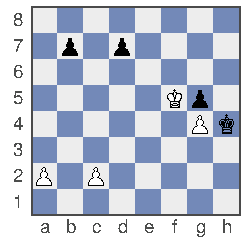
\includegraphics[width=0.7\columnwidth]{figures/star2_textbook.pdf}
\caption{Textbook $\nim{2}$ candidate \pos{W a2 c2 / B b7 d7}, with the kings frozen by the tr\'ebuchet on
files f--h (ordinary board). It is $\nim{2}$ under the textbook passed-pawn test and $\game{2\pm1}{-2\pm1}$
under the e.p.-aware test.}
\label{fig:star2_textbook}
\end{figure}

Fig.~\ref{fig:star2_textbook} shows \pos{W a2 c2 / B b7 d7} on files a--d, with the kings frozen by the
tr\'ebuchet on files f--h. Under the textbook passed-pawn test and the count rule, it is the only position of
value $\nim{k}$ with $k\ge2$ in the flat census. If white (Left) moves first, a2--a4 leaves $\star$ and c2--c4
leaves the zero game; the single steps a2--a3 and c2--c3 are worse. The position is symmetric (turn the board
around and swap the colors), so black (Right) has the same choice: d7--d5 leaves $\star$ and b7--b5 leaves $0$.
Thus $G=\game{0,\star}{0,\star}=\nim{2}$. The value is the same under the mover rule and with e.p.\ off, and it is
$0$ under the opponent rule \lab{C2}.

The weak point is black's plan b7--b5 and b5--b4. The textbook test answers b5--b4 with a2--a4: no black pawn
stands in front of the a-pawn, so the test calls it passed and scores $+\BIG$. In chess, black simply plays b4$\times$a3
en passant. Under the e.p.-aware test of Section~\ref{sec:rules}, the position after b5--b4,
\pos{W a2 c2 / B b4 d7}, is no longer a white win but a black one. So b7--b5 is worth $-2\pm1$ for black and, by
symmetry, c2--c4 is worth $2\pm1$ for white. The other moves, such as a2--a4 and d7--d5 (both still to $\star$),
are dominated or reversible. Hence
\begin{equation}
G=\game{2\pm1}{-2\pm1}\qquad\lab{C2},
\end{equation}
a hot game with mean $0$ and temperature $2$. The candidate's $\nim{2}$ rested on one double step, a2--a4 past
a black pawn on b4, that the textbook test counts as passed one move too early.

\subsection{No \texorpdfstring{$\nim{2}$}{*2} With Six Pawns or Fewer}

\begin{theorem}[Census; \lab{C2}]\label{thm:census}
Consider the flat census: ordinary boards with $8$ ranks and $1$ to $4$ files, with at most six pawns
($231{,}071$ records standing for $459{,}443$ positions). Under the count rule with the e.p.-aware test and
e.p.\ on, no position has value $\nim{k}$ with $k\ge2$. The census has $6{,}724$ positions of value $0$ and
$4{,}042$ of value $\star$.
\end{theorem}

Three independent programs give this result (Section~\ref{sec:verify}). Our CGT engine and a separate C
solver, which tests whether $G+\nim{k}$ is a second-player win, agree on every record. A third solver, written
from the rules alone, finds no $\nim{k}$ with $2\le k\le 292$ among $793{,}299$ labeled placements. Every
position in scope has birthday at most $292$ (at most $36$ pawn moves before a decided position of birthday
$\BIG=256$), so no larger nimber can occur. Under the textbook test the same census has $6{,}470$ zeros,
$3{,}891$ stars and the one $\nim{2}$ above. The e.p.-aware test removes that $\nim{2}$ and creates none, so in
this scope the only route to $\nim{2}$ was the en passant artifact.

\subsection{\texorpdfstring{$\nim{2}$}{*2} Returns With Seven Pawns}

\begin{theorem}[$\nim{2}$ with seven pawns; \lab{C2}]\label{thm:star2seven}
Under the count rule with the e.p.-aware test and e.p.\ on, position~A, \pos{W a4 b3 d2 d3 / B a7 b7 c5}, and
position~B, \pos{W b4 c2 d2 / B a6 a7 c6 d5}, both on files a--d of the ordinary board, have value $\nim{2}$.
Both are also $\nim{2}$ under the mover rule and under the textbook test. Neither is $\nim{2}$ with e.p.\ off or
under the opponent rule. Both embed legally beside the tr\'ebuchet on files f--h.
\end{theorem}

Three programs give $\nim{2}$ in every setting the theorem claims: our CGT engine (on 4- and 8-file boards), the
C scanner that found the two positions, and the independent whole-board solver.

\begin{figure}[!t]
\centering
\begin{subfigure}{0.48\columnwidth}\centering
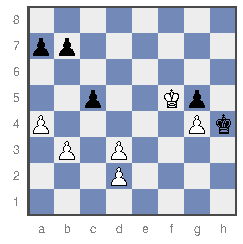
\includegraphics[width=\linewidth]{figures/star2_seven_a.pdf}
\caption{Position A}\label{fig:star2_seven_a}
\end{subfigure}\hfill
\begin{subfigure}{0.48\columnwidth}\centering
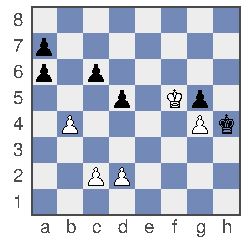
\includegraphics[width=\linewidth]{figures/star2_seven_b.pdf}
\caption{Position B}\label{fig:star2_seven_b}
\end{subfigure}
\caption{Seven-pawn positions of value $\nim{2}$ (count rule, e.p.-aware test), each beside the tr\'ebuchet on
files f--h (ordinary board). (a) Position A, \pos{W a4 b3 d2 d3 / B a7 b7 c5}. (b) Position B,
\pos{W b4 c2 d2 / B a6 a7 c6 d5}.}
\label{fig:star2_seven}
\end{figure}

In position A (Fig.~\ref{fig:star2_seven_a}), if white (Left) moves first, a4--a5 leaves the zero game. The move
d3--d4 attacks c5, and every black reply except c5$\times$d4 loses at once; after c5$\times$d4, white continues b3--b4 and
reaches $\star$. So d3--d4 is a reversible move, and it counts as a move to $\star$. White's last move, b3--b4,
loses to c5$\times$b4, which gives black a passed pawn. If black (Right) moves first, a7--a5 leaves $0$ and b7--b6
leaves $\star$. Black's other moves are worse: a7--a6 and b7--b5 are dominated, and c5--c4 loses the pawn to a
capture on c4 that frees white's d-pawn. Thus $G=\game{0,\star}{0,\star}=\nim{2}$.

In position B (Fig.~\ref{fig:star2_seven_b}), if white moves first, d2--d4 leaves $0$ and c2--c3 leaves
$\star$. The moves d2--d3 and c2--c4 are dominated, and b4--b5 loses to a6$\times$b5. Black has three moves. d5--d4
leaves $0$. The move a6--a5 attacks b4: every white reply except b4$\times$a5 loses at once, and after b4$\times$a5 black
continues c6--c5 and reaches $\star$. So, as in A, a reversible move counts as a move to $\star$. Finally,
c6--c5 loses to b4$\times$c5. Thus $G=\nim{2}$ again.

\begin{table}[!t]
\centering
\caption{Values of the Three $\nim{2}$ Positions in the Model Settings}
\label{tab:star2_settings}
\footnotesize
\setlength{\tabcolsep}{4pt}
\begin{tabular}{@{}lccc@{}}
\toprule
Race rule, passed-pawn test & Candidate & A & B\\
\midrule
count, e.p.-aware & $\game{2\pm1}{-2\pm1}$ & $\nim{2}$ & $\nim{2}$\\
mover, e.p.-aware & $\game{2\pm1}{-2\pm1}$ & $\nim{2}$ & $\nim{2}$\\
count or mover, textbook & $\nim{2}$ & $\nim{2}$ & $\nim{2}$\\
count or mover, e.p.\ off & $\nim{2}$ & not $\nim{2}$ & not $\nim{2}$\\
opponent, textbook or e.p.\ off & $0$ & not $\nim{2}$ & not $\nim{2}$\\
\bottomrule
\end{tabular}
\end{table}

Table~\ref{tab:star2_settings} compares the settings (e.p.\ on unless stated; every entry \lab{C2}). The
candidate and the new positions fail in opposite places. The candidate needs the textbook test but survives
e.p.\ off. Positions A and B do not depend on the passed-pawn test at all, but they need en passant: with e.p.\
off neither is $\nim{2}$.

\begin{figure}[!t]
\centering
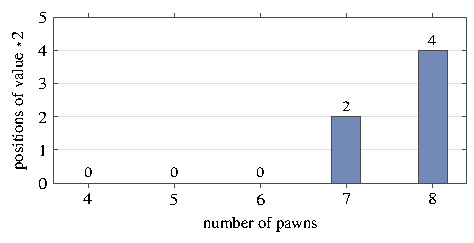
\includegraphics[width=\columnwidth]{figures/star2_by_pawns.pdf}
\caption{Number of $\nim{2}$ positions by number of pawns, on ordinary boards of width at most four (count rule,
e.p.-aware test). The bars for four to six pawns are \lab{C2}. The bars for seven and eight pawns are \lab{C1}
as counts, and every position they count was re-checked \lab{C2}.}
\label{fig:star2_by_pawns}
\end{figure}

\subsubsection{Scope}
Fig.~\ref{fig:star2_by_pawns} counts $\nim{2}$ positions by number of pawns on ordinary boards of width at most
four. With four to six pawns there are none (Theorem~\ref{thm:census}). With seven pawns there are exactly the
two above, and with eight pawns there are four. These two counts come from one exhaustive scan of
$5{,}503{,}282$ root positions, so as claims of completeness they are \lab{C1}; every position the scan reported
was re-checked by our engine \lab{C2}. Theorems~\ref{thm:census} and~\ref{thm:star2seven} together show that
seven is the least number of pawns in a $\nim{2}$ on ordinary boards of width at most four \lab{C2}.

\subsubsection{Five files}
We also know three eight-pawn positions on five files that are $\nim{2}$ on the ordinary board \lab{C2}, both
as a sum of components and on the whole board (Section~\ref{sec:sums}): \pos{W a3 b3 c2 e2 / B a6 c5 d5 e3},
\pos{W a4 b3 c2 d2 / B a7 b6 c7 e4} and \pos{W a6 b4 c4 e3 / B a7 c7 d6 e6}. They come from a scan of
eight-pawn rings on the 5-file cylinder $\cyl{5}$, which finds $14$ rings of value $\nim{2}$ \lab{C1}, each
confirmed by our engine. Opened onto files a--e of the ordinary board, $11$ of the $14$ change value and only
these three stay $\nim{2}$. No $\nim{3}$ or higher nimber occurs under the count rule with the e.p.-aware test
in any scope we searched \lab{C1}.

\subsubsection{What this answers}
Within the model, with the kings frozen by the tr\'ebuchet, the count rule and the e.p.-aware test, the
$\nim{2}$ question has a positive answer: there are king-and-pawn positions on the ordinary $8\times8$ board of
value $\nim{2}$. Elkies' higher nimbers live on larger boards~\cite{Elkies2002}. Positions A and B use four files of
the 8-rank board, no officers and seven pawns, and they hold under the stricter passed-pawn test that removed the
candidate. The answer has limits: it fails under the opponent rule and with e.p.\ off, the completeness counts
for seven and eight pawns are \lab{C1}, and the value is a model value. Whether real chess agrees is the
subject of Section~\ref{sec:real}.
